\section{Estudios y enfoques alterativos}

A continuación, se han evaluado dos enfoques alternativos de control difuso de la calidad del ambiente interior, para más adelante hacer un estudio comparativo de los tres.

\subsection{Control fuzzy de sistemas HVAC optimizado con algoritmos genéticos}

Este trabajo, realizado por un investigador de la Universidad de Jaén (Rafael Alcalá) y cuatro de la Universidad de Granada (José M. Benitez, Jorge Casillas, Oscar Cordón y Raúl Pérez) combina control difuso con algoritmos genéticos para optimizar los sistemas HVAC, mejorando la eficiencia energética y el confort \parencite{alcala2003fuzzy}.

El estudio se centró en el control de sistemas HVAC en dos sitios de prueba reales, con el objetivo de optimizar tanto el rendimiento energético como las condiciones de confort interior. Estos sitios incluían un centro de investigación en Francia y una instalación privada. Cada uno tenía características específicas, como sistemas HVAC de diferente configuración, lo que presentaba un desafío adicional para diseñar un controlador adaptable y eficiente. Los expertos proporcionaron modelos térmicos detallados para ambos sitios, ajustados a las condiciones climáticas y de ocupación específicas de cada temporada.

\subsubsection{Diseño del controlador difuso}

El controlador difuso fue diseñado para manejar múltiples criterios, como el confort térmico, la calidad del aire interior y el consumo de energía, usando una base de reglas construida con la experiencia de expertos. Además, se utilizaron funciones de pertenencia triangulares para simplificar el proceso de inferencia y mejorar la manejabilidad del sistema.

A diferencia del estudio principal que se trata en este documento, este proyecto también integró algoritmos genéticos (AG) para afinar automáticamente los parámetros del controlador difuso. Estos AG optimizaron las bases de conocimiento ajustando las funciones de pertenencia para mejorar el rendimiento del sistema bajo diferentes condiciones operativas. El método propuesto recibió el nombre de \textit{Weighted Multi-Criteria Steady-State Genetic Algorithm} (WMC-SSGA), cuyo comportamiento viene reflejado en la \autoref{fig:flowchart-ga}.

\begin{figure}[H]
	\centering
	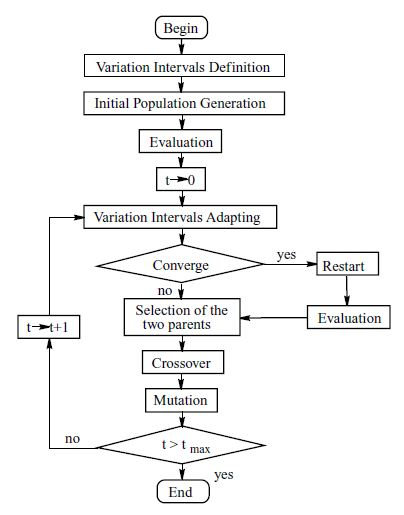
\includegraphics[width=0.45\textwidth]{imgs/flowchart-ga.JPG}
	\caption{Ddiagrama de flujo del algoritmo WMC-SSGA \parencite{alcala2003fuzzy}.}
	\label{fig:flowchart-ga}
\end{figure}

No se va a entrar en detalle con el funcionamiento del algoritmo genético, pero se podría resumir de la siguiente manera:

El WMC-SSGA comienza con la generación de una población inicial dentro de unos límites. Estas soluciones potenciales codifican parámetros para el controlador difuso, que serán evaluadas por el algoritmo basándose en una función objetivo multicriterio ponderada (con indicadores como minimizar el consumo energético y mantener los niveles de confort). Si no hay suficiente mejora, se ajustan los límites, y después, se seleccionan las mejores soluciones (padres), que se combinan y modifican para crear nuevas soluciones. Este proceso se repite de forma iterativa, evaluando y mejorando las soluciones hasta llegar a un límite o encontrar una solución lo suficientemente buena.

El método anterior contrasta con el FLC unificado, que carece de capacidades de autoajuste y depende únicamente de reglas definidas por expertos.


El controlador difuso presenta una estructura jerárquica, diseñada para procesar múltiples variables y tomar decisiones complejas optimizando el rendimiento del sistema HVAC. Esta estructura se organiza en módulos jerárquicos, donde cada nivel se encarga de tareas específicas y alimenta al siguiente. Se muestra un ejemplo en la \autoref{fig:fuzzy-genetics-functions}.

En la primera capa, se procesan variables básicas como las entradas del índice de control térmico (\textit{PMV}), el valor del PMV anterior (\textit{PMV t-1}), la diferencia entre la temperatura exterior y la interior (\textit{Tout-Tin}) y la posición de la válvula antes del ajuste (\textit{Valve old position}). 

Las flechas entre módulos indican el flujo de la información, señalando cómo los módulos de niveles inferiores sirven para calcular valores que son utilizados como entradas por los niveles superiores. Por ejemplo, partiendo de la \textit{PMV} y \textit{PMV t-1}, se obtiene la preferencia térmica (\textit{Thermal preference}) basada en las condiciones actuales del ambiente. Y esta variable, que pertenece a la segunda capa, puede utilizarse con la \textit{Tout-Tin} para obtener calor requerido (\textit{Required heat}). Este último es necesario en la tercera capa para, junto con la anterior posición de la válvula y la prioridad térmica/energética, poder calcular tanto la nueva posición de la válvula como la velocidad del ventilador del sistema HVAC.

\begin{figure}[H]
	\centering
	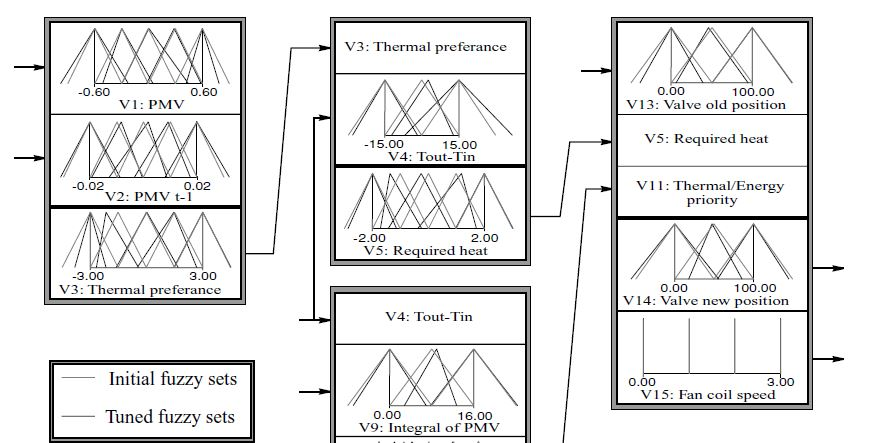
\includegraphics[width=0.95\textwidth]{imgs/fuzzy-genetics-functions.JPG}
	\caption{Diagrama de módulos jerárquicos y funciones de pertenencia \parencite{alcala2003fuzzy}.}
	\label{fig:fuzzy-genetics-functions}
\end{figure}

Las optimizaciones fruto del algoritmo genético vienen reflejadas en la \autoref{fig:fuzzy-genetics-functions} mediante las líneas negras de las gráficas, en contraste con las grises, que representan la configuración original del sistema. Tras la optimización, las funciones muestran ligeros desplazamientos y ajustes en sus picos y bordes, adaptándose mejor a los datos del modelo, ya que estos cambios buscan maximizar la precisión y robustez del sistema.

Asimismo, a diferencia del estudio anterior, en este se ha seguido el \textit{Modo B - FITA} (\textit{First Infer Then Aggregate}). <<En este modo de trabajo, se considera individualmente la contribución de cada conjunto difuso inferido y la acción precisa final se obtiene mediante algún tipo de operación efectuada sobre un valor preciso
característico obtenido a partir de cada conjunto difuso individual. De este modo, se
evita el calculo del conjunto difuso final, lo que ahorra una gran cantidad de
tiempo de cálculo>> \parencite{peregrin2000integracion}. Dicho en otras palabras, cada conjunto difuso resultante de una regla se defuzzifica individualmente, y posteriormente, se utiliza una técnica para combinar los valores crisp obtenidos y así poder producir la salida final.

Para la defuzzificación, en lugar del cálculo del centroide, se ha empleado la técnica \textit{MOM} (\textit{Mean of Maxima}) o media de los máximos, en el que se seleccionan todos los puntos del conjunto difuso de salida donde la función de pertenencia alcanza su valor máximo, para luego calcular el promedio aritmético de esos puntos máximos.

\begin{figure}[H]
	\centering
	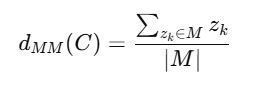
\includegraphics[width=0.33\textwidth]{imgs/mom.JPG}
	\caption{Fórmula de Mean of Maxima (MOM) \parencite{klir1996fuzzy}.}
	\label{fig:mom}
\end{figure}

En la \autoref{fig:mom}, se considera un conjunto $M$ de valores crisp ($z_k$) que tienen el grado de pertenencia máximo dentro del conjunto difuso $C$. 

\subsubsection{Pruebas}

Se llevaron a cabo experimentos tanto en simulaciones como en entornos reales. Los primeros permitieron evaluar durante períodos de 10 días las distintas configuraciones del controlador bajo condiciones climáticas específicas; mientras que los segundos proporcionaron validación en condiciones más realistas. Los resultados se compararon con un controlador convencional On-Off y con versiones iniciales no optimizadas del FLC para medir la mejora alcanzada.

\subsubsection{Resultados y conclusiones}

Al igual que el controlador difuso unificado, los resultados de este estudio mostraron mejoras significativas en comparación con los controladores tradicionales.

En términos de eficiencia energética, en este estudio se lograron ahorros de hasta un 20\% en algunos casos gracias al uso de algoritmos genéticos, mientras que los parámetros de confort se mantuvieron dentro de los rangos deseados con fluctuaciones mínimas. Estos resultados sugieren que la integración de técnicas avanzadas de optimización puede potenciar aún más la eficacia de los controladores difusos.

\subsection{Sistema de inferencia difusa centrado en la evaluación de IEQ}

El sistema propuesto por Karol Jabłonski y Tomasz Grychowski, miembros de una universidad polaca, se diseñó para evaluar las condiciones ambientales interiores en un edificio mediante un sistema de sensores y un módulo de inferencia difusa. Similar al primer estudio, este sistema se enfocó en múltiples parámetros como temperatura, humedad y CO2, pero también integró otros factores como iluminación, ruido y olores, proporcionando una evaluación más completa del confort interior \parencite{jablonski2018fuzzy}.

El estudio no describe un controlador difuso en el sentido clásico (es decir, un sistema que toma decisiones para regular un proceso dinámico), sino más bien un sistema de inferencia difusa diseñado para evaluar y calificar el confort ambiental en interiores. Aunque emplea lógica difusa y comparte componentes clave de un controlador difuso (como funciones de pertenencia, reglas difusas y defuzzificación), su propósito es diferente.

Dicho esto, el sistema podría evolucionar hacia un controlador difuso si sus salidas fueran utilizadas para ajustar automáticamente dispositivos como sistemas HVAC.

\subsubsection{Diseño del sistema difuso}

Este estudio adoptó un sistema híbrido de inferencia difusa para procesar múltiples índices, utilizando una estructura modular con subsistemas independientes para manejar los distintos parámetros.

La \autoref{fig:fuzzy-inference-system-diagram} representa el funcionamiento del sistema de inferencia difusa, que se distingue por su enfoque integral, al combinar múltiples parámetros ambientales mediante subsistemas especializados que contribuyen a una evaluación global del confort. 

Las variables monitoreadas incluyen temperatura del aire, temperatura de globo negro, humedad relativa, densidad de CO2, iluminación, ruido y olores, que se procesan a través de módulos de inferencia difusa para estimar diferentes índices de confort. Cada uno de estos índices (confort térmico, frescura del aire y fatiga) es calculado de forma independiente en tres subsistemas, y luego integrado en un módulo principal (confort general) que genera una evaluación global del confort percibido.

Así, a diferencia de los otros dos sistemas que se centran en un conjunto más reducido de variables, este enfoque incluye factores adicionales como olores y ruido, que pueden tener un impacto significativo en la percepción del confort. Además, el sistema consta de 92 reglas difusas, distribuidas entre 4 subsistemas principales, lo que contrasta con un enfoque unificado, que habría requerido hasta 2400 reglas para cubrir todas las combinaciones posibles de entradas.

\begin{figure}[H]
	\centering
	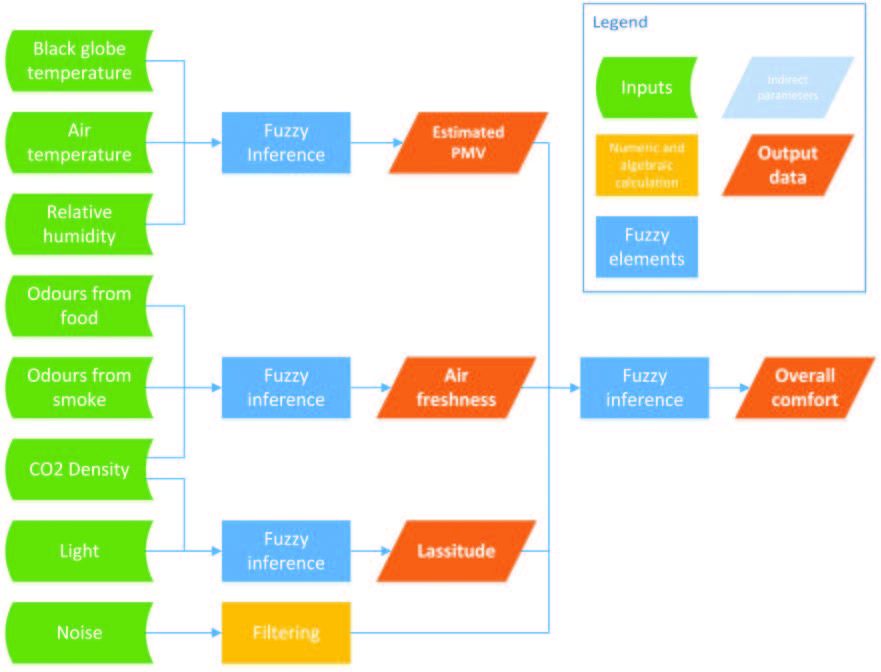
\includegraphics[width=0.75\textwidth]{imgs/fuzzy-inference-system-diagram.JPG}
	\caption{Diagrama del sistema de inferencia difusa \parencite{jablonski2018fuzzy}.}
	\label{fig:fuzzy-inference-system-diagram}
\end{figure}

En este estudio se han utilizado funciones de pertenencia triangulares para las salidas y trapezoidales para algunas entradas. Se muestra un ejemplo en la \autoref{fig:fuzzy-2-membership-lassitude-freshness}. 

\begin{figure}[H]
	\centering
	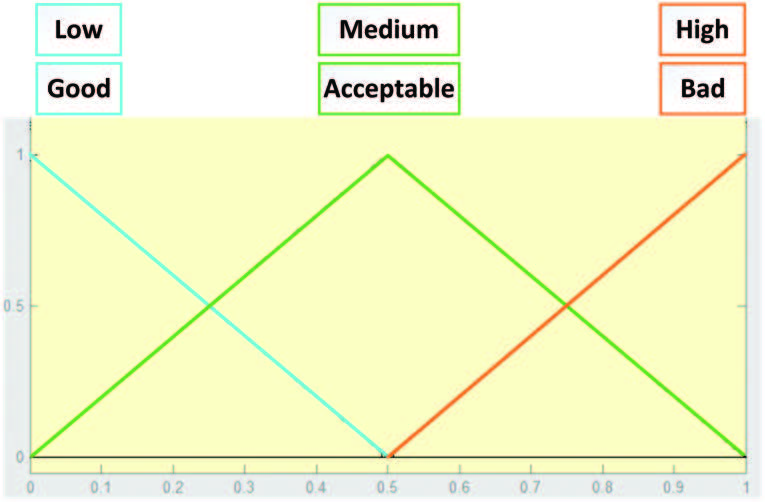
\includegraphics[width=0.5\textwidth]{imgs/fuzzy-2-membership-lassitude-freshness.JPG}
	\caption{Funciones de pertenencia de la fatiga y frescura \parencite{jablonski2018fuzzy}.}
	\label{fig:fuzzy-2-membership-lassitude-freshness}
\end{figure}

Además, este sistema destaca por implementar un módulo de inferencia en \textit{LabVIEW}, diseñando desde cero los bloques de fuzzificación, inferencia y defuzzificación, mientras que en otros estudios se utilizaron herramientas estándar o adaptaciones de controladores PID.

\subsubsection{Pruebas}

Las pruebas en este sistema se realizaron en un entorno real, con mediciones de confort en diferentes condiciones, incluyendo variaciones en ocupación y ventilación en múltiples escenarios. 

Durante las pruebas, se realizaron encuestas para validar los índices calculados por el sistema, permitiendo alinear las percepciones humanas con las salidas del sistema y obteniendo una alta concordancia entre ambas. El enfoque anterior no está presente en los otros dos estudios, donde la validación se centró más en la comparación con sistemas tradicionales o en el análisis de la eficiencia energética.

\subsubsection{Resultados y conclusiones}

En la \autoref{fig:fuzzy-inference-system-results}, se comparan las salidas del sistema difuso con encuestas subjetivas en los cuatro aspectos del confort ambiental definidos por los subsistemas. Los resultados muestran que el sistema sigue tendencias similares a las percepciones humanas, con picos y descensos relacionados con cambios en las condiciones ambientales, aunque es más continuo y menos variable que las encuestas. Esto valida la capacidad del sistema para evaluar objetivamente el confort, reflejando correctamente los efectos de factores como temperatura, iluminación y concentración de CO2.

\begin{figure}[H]
	\centering
	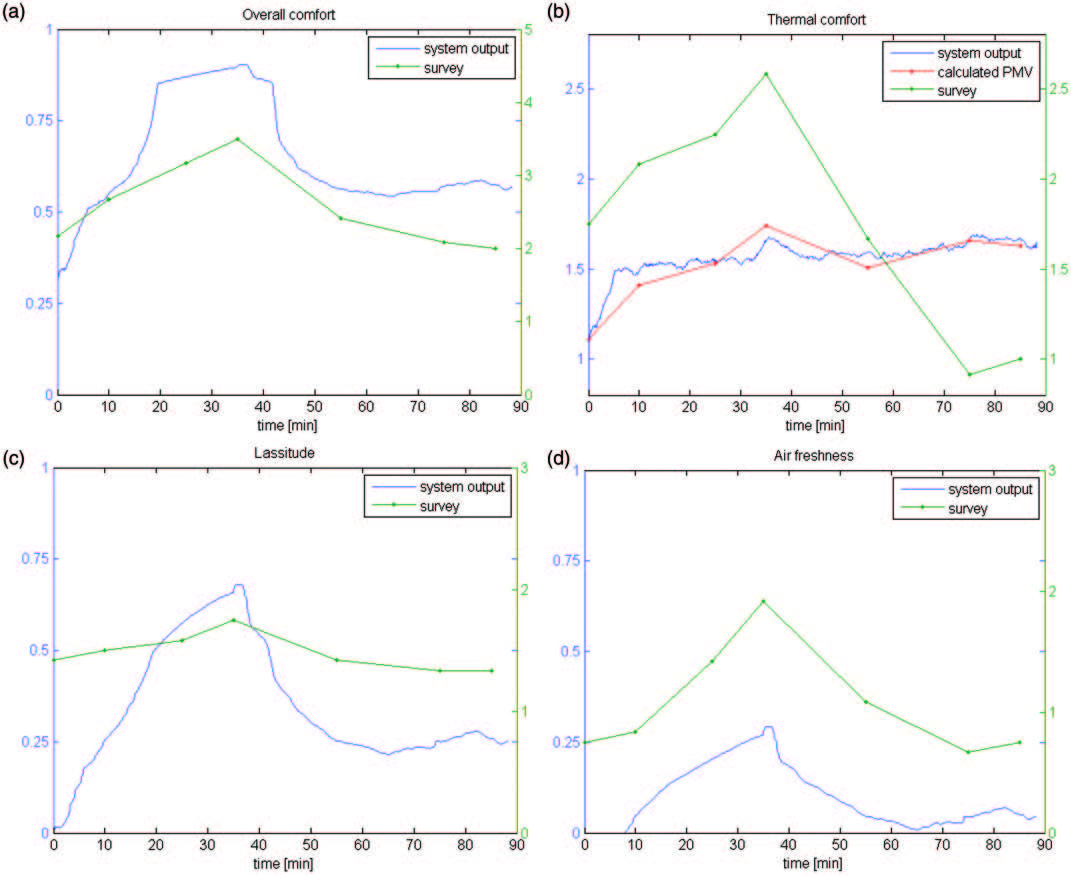
\includegraphics[width=0.76\textwidth]{imgs/fuzzy-inference-system-results.JPG}
	\caption{Resultados de las encuestas y medidas del sistema \parencite{jablonski2018fuzzy}.}
	\label{fig:fuzzy-inference-system-results}
\end{figure}

Este enfoque destaca por la detección de eventos específicos como la presencia de alimentos o cambios en la ocupación. De esta forma, este sistema amplía el rango de variables monitoreadas y evaluadas, proporcionando una evaluación más centrada en todo aquello que define IEQ.

Como ventajas adicionales, dividir un sistema difuso en subsistemas reduce drásticamente la complejidad al evitar el crecimiento exponencial ($n^m$, siendo $n$ es el número de valores de entrada y $m$ el número de entradas) de reglas que ocurriría en un sistema unificado, donde cada entrada y sus combinaciones requieren cobertura. Esto hace que el diseño sea más manejable y ajustable. Además, la modularidad permite mejorar o expandir cada subsistema de forma independiente, sin afectar al resto; por ejemplo, al añadir un nuevo sensor solo se ajusta el subsistema correspondiente. También mejora la eficiencia computacional, ya que cada subsistema realiza cálculos más simples, permitiendo respuestas rápidas a los cambios ambientales.

Aunque dividir un sistema difuso en subsistemas ofrece claras ventajas, también puede presentar algunas desventajas en comparación con el enfoque unificado. Una de las principales limitaciones es la pérdida de interacción directa entre todas las variables de entrada. Al segmentar las entradas en módulos, las interacciones complejas que podrían influir en el resultado general pueden no ser capturadas de manera precisa, ya que cada subsistema procesa solo un subconjunto de las variables. Además, requiere una fase adicional de integración para combinar las salidas de los subsistemas en un resultado global, lo que puede introducir incertidumbre o simplificaciones adicionales. Finalmente, aunque se reduce la complejidad computacional, un sistema unificado podría ser más eficiente en aplicaciones donde el hardware es suficientemente potente, ya que permite procesar todas las combinaciones posibles en una sola etapa sin necesidad de combinar resultados.

\subsection{Comparaciones entre los tres estudios}

Las comparaciones entre FLCs diseñados se han realizado en base a cinco aspectos generales:

\begin{table}[H]
	\centering
	\renewcommand{\arraystretch}{1.5}
	\begin{tabular}{|p{2.5cm}|p{4cm}|p{4cm}|p{4cm}|}
		\hline
		\rowcolor{lightgray}
		\textbf{Aspecto} & \textbf{Controlador difuso unificado} & \textbf{Controlador con algoritmos genéticos} & \textbf{Sistema de inferencia difusa} \\ \hline
		
		\textbf{Variables controladas} & 
		Temperatura, humedad, CO2, iluminación & 
		Temperatura, humedad, con optimización dinámica & 
		Temperatura, humedad, CO2, iluminación, ruido, olores \\ \hline
		
		\textbf{Enfoque metodológico} & 
		Controlador difuso clásico con reglas definidas por expertos. FLC supervisa PIDs para HVAC & 
		Integración de algoritmos genéticos para optimizar automáticamente reglas y funciones de pertenencia & 
		Arquitectura modular con subsistemas independientes. Implementación en LabVIEW \\ \hline
		
		\textbf{Pruebas y validación} & 
		Pruebas en una habitación piloto controlada, comparando con controlador reactivo & 
		Simulaciones y pruebas en múltiples entornos reales bajo diferentes condiciones estacionales & 
		Pruebas en entornos ocupados reales, correlacionando resultados con encuestas de usuarios \\ \hline
		
		\textbf{Objetivo principal} & 
		Optimizar el confort interior y la eficiencia energética en sistemas HVAC & 
		Equilibrio dinámico entre confort y eficiencia energética & 
		Evaluación integral del confort interior basado en múltiples índices \\ \hline
		
		\textbf{Aplicación recomendada} & 
		Escenarios con reglas de confort bien definidas, simplicidad y robustez & 
		Entornos donde se requiere máxima eficiencia energética y adaptabilidad & 
		Edificios donde la percepción humana del confort es crítica \\ \hline
	\end{tabular}
	\caption{Comparación de tres estudios sobre controladores difusos para IEQ.}
	\label{tab:comparacion}
\end{table}

En conjunto, estos tres enfoques destacan la flexibilidad de los controladores difusos y su capacidad para adaptarse a distintas necesidades y restricciones operativas.

La elección entre estos enfoques dependerá del contexto de aplicación y los objetivos específicos, como si se busca mayor integración en sistemas existentes o una evaluación más detallada de los parámetros de confort.